\chapter{Apprendimento su dati strutturati e grafi}\label{ch-21}

L'ultima lezione del corso è un'introduzione avanzata
all'\textbf{apprendimento in domini strutturati} (SD, \emph{Structured
Domains}) e in particolare all'\textbf{apprendimento su grafi} con le
\textbf{Deep Graph Networks} (DGN). È anche una panoramica delle
ricerche del gruppo CIML di Pisa, che ha contribuito in modo
pionieristico a questo campo. Le domande guida: si può fare deep
learning sui grafi in modo \textbf{efficiente} (senza un addestramento
completamente \emph{end-to-end})? La \textbf{profondità} nelle DGN
serve, ma causa problemi: perché? Qual è il rapporto tra profondità dei
modelli e difficoltà di addestramento?

\section{Perché dati strutturati e
grafi}\label{perchuxe9-dati-strutturati-e-grafi}

\textbf{Perché i dati hanno relazioni.} Esempi di grafi e reti:

\begin{itemize}
\tightlist
\item
  astrazioni di immagini e reti per la comprensione di scene;
\item
  \textbf{social network}, \textbf{knowledge graph};
\item
  analisi sintattica del linguaggio (alberi di parsing);
\item
  reti di trasporto (ad esempio la previsione del traffico su Google
  Maps, di DeepMind);
\item
  \textbf{piccole molecole} (drug design), reti biologiche (proteine);
\item
  termini logici, modellazione di reti cerebrali.
\end{itemize}

\begin{figure}[htbp]
\centering
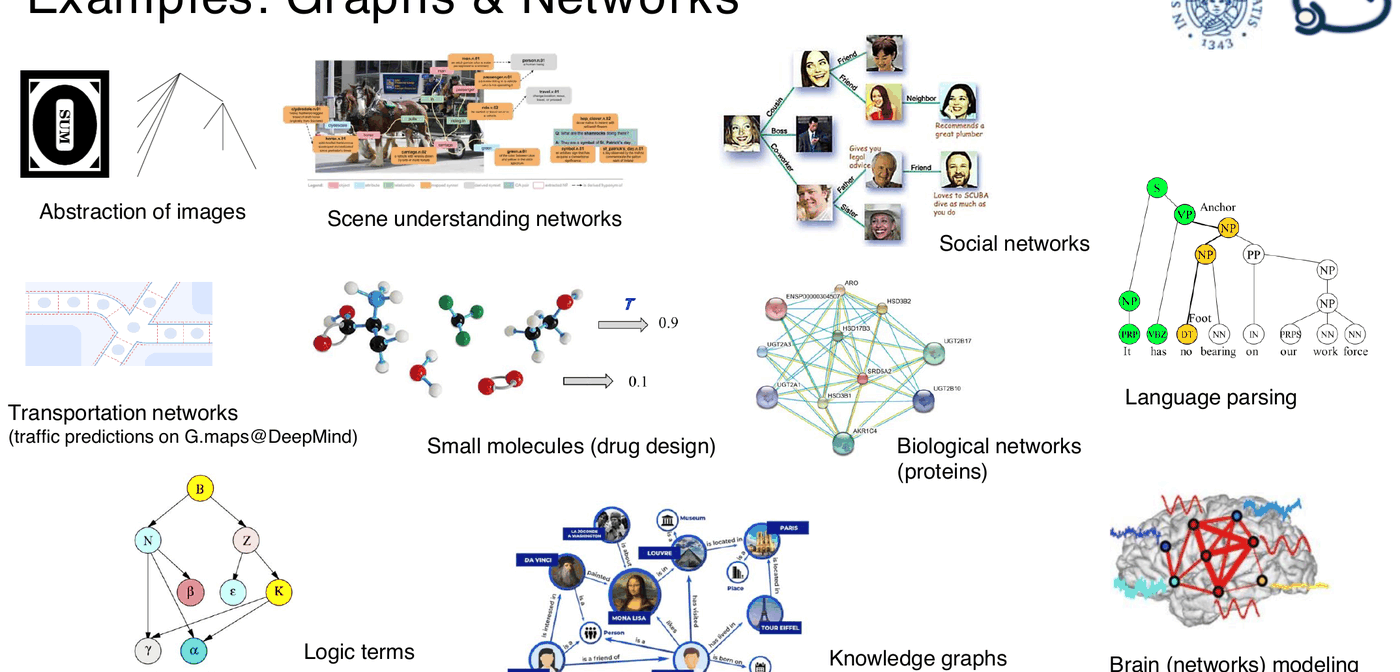
\includegraphics[width=0.91\linewidth,height=0.42\textheight,keepaspectratio]{images/21-sdl_esempi-grafi.png}
\caption{Esempi di grafi e reti in domini diversi.}
\end{figure}

\subsection{Lo scenario}\label{lo-scenario}

\begin{figure}[htbp]
\centering
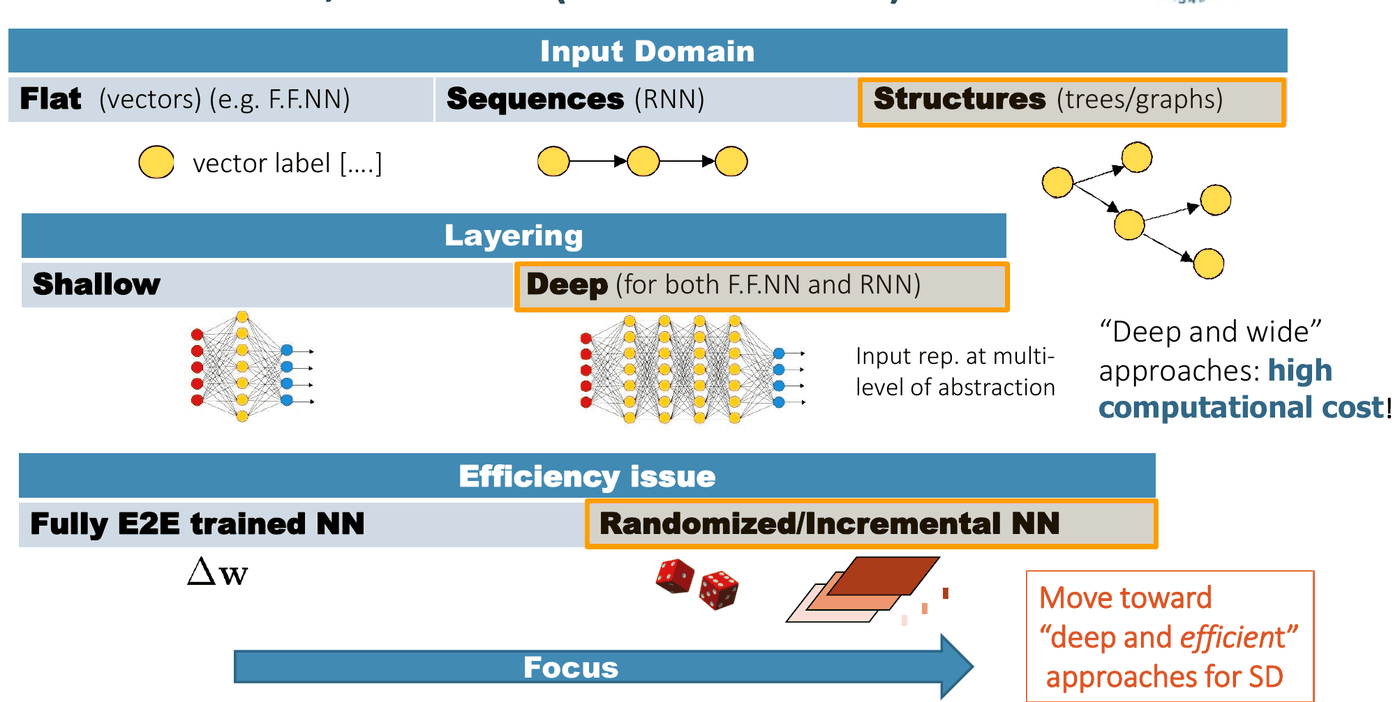
\includegraphics[width=0.89\linewidth,height=0.42\textheight,keepaspectratio]{images/21-sdl_scenario.png}
\caption{Lo scenario: dal dominio di input piatto a quello strutturato, da
modelli superficiali a profondi, dall'addestramento end-to-end a quello
randomizzato o incrementale. L'obiettivo è ottenere approcci ``profondi
ed efficienti'' per i dati strutturati.}
\end{figure}

Il corso ha seguito questa progressione: dai \textbf{vettori} (reti
feedforward) alle \textbf{sequenze} (RNN) alle \textbf{strutture}
(alberi, grafi). Gli approcci profondi e ``larghi'' (\emph{deep and
wide}) rappresentano l'input su più livelli di astrazione ma hanno un
alto costo computazionale; le reti \textbf{randomizzate} o
\textbf{incrementali} offrono l'efficienza.

\subsection{Un po' di storia}\label{un-po-di-storia}

Le reti neurali per dati strutturati hanno una storia in gran parte
\textbf{italiana}:

\begin{itemize}
\tightlist
\item
  dalla fine degli anni '90, le \textbf{reti neurali ricorsive} per
  alberi e grafi aciclici orientati (Sperduti, Starita, Frasconi, Gori,
  Hammer, Micheli, Bianchini, Scarselli, Hagenbuchner\ldots): reti
  ricorsive (1997--2000), Cascade Correlation per strutture, SOM per
  strutture (2003--2005), Hidden Tree Markov Model bottom-up (2012),
  Tree ESN e reservoir computing profondo per alberi (2010--2018);
\item
  l'estensione ai \textbf{grafi generali}, pionieristica tra Pisa e
  Siena (2005--2009), con due approcci:

  \begin{enumerate}
  \def\labelenumi{\arabic{enumi}.}
  \tightlist
  \item
    \textbf{ricorsivi}: \textbf{GNN} (Scarselli et al., 2009) e
    \textbf{GraphESN} (Gallicchio, Micheli, 2010);
  \item
    \textbf{a strati / convoluzionali}: \textbf{NN4G} (Micheli, 2009) in
    versione costruttiva, poi proseguito come reti convoluzionali per
    grafi (GCN, ecc.).
  \end{enumerate}
\end{itemize}

Dal 2015 è un'area in \textbf{esplosione} a livello mondiale, con decine
di articoli in tutte le principali conferenze e applicazioni reali,
sotto nomi diversi: \emph{Graph Representation Learning}, \emph{learning
on graphs}, \emph{deep learning for graphs}, \emph{Graph Neural
Networks} (GNN), \emph{Graph Convolutional Networks} (GCN), e il quadro
delle \textbf{Deep Graph Networks} (DGN; Bacciu, Errica, Micheli, Podda,
2020).

\section{Deep Graph Networks}\label{deep-graph-networks}

\subsection{I grafi considerati}\label{i-grafi-considerati}

Si considerano \textbf{grafi etichettati}: ogni \textbf{nodo} (vertice)
\(v\) ha un'\textbf{etichetta vettoriale} \(\mathbf{l}(v)\) (es.
\([1, 0, 1, 0{,}7]\)), ogni \textbf{arco} (link) può avere un'etichetta
(es. una posizione) e può essere orientato; possono esserci
\textbf{cicli}. \(A\) è la \textbf{matrice di adiacenza} del grafo.

\begin{figure}[htbp]
\centering
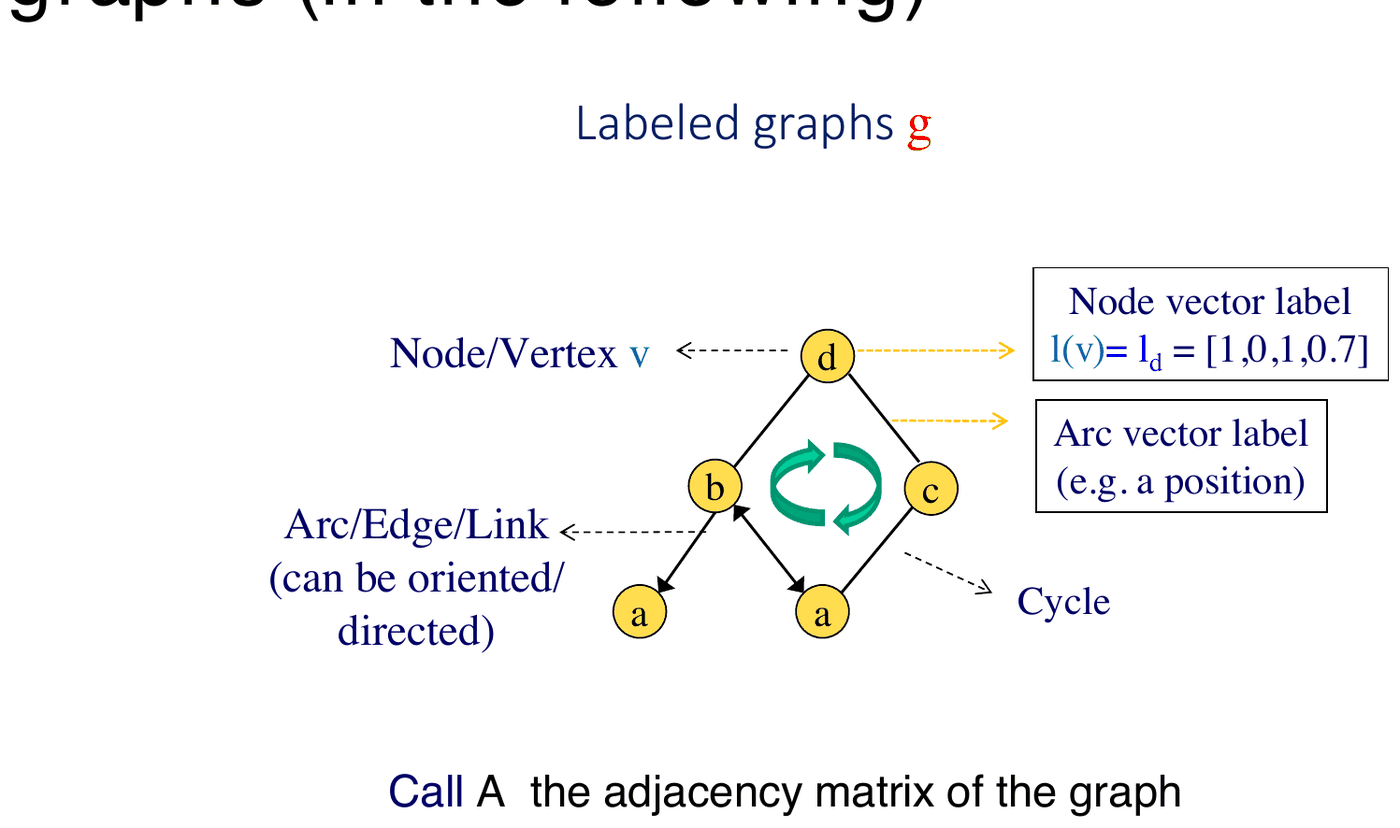
\includegraphics[width=0.63\linewidth,height=0.42\textheight,keepaspectratio]{images/21-sdl_grafo-etichettato.png}
\caption{Un grafo etichettato: etichette vettoriali su nodi e archi, possibili
cicli.}
\end{figure}

\subsection{Il problema della
rappresentazione}\label{il-problema-della-rappresentazione}

Non esisteva un modo \textbf{sistematico} (valido per qualunque task)
per estrarre feature o metriche di relazione tra esempi strutturati. È
un'istanza del \textbf{representation learning}, estesa ai domini
strutturati.

\begin{itemize}
\tightlist
\item
  Le rappresentazioni basate su \textbf{feature} sono incomplete o
  fortemente dipendenti dal task (ad esempio gli indici topologici in
  chimica).
\item
  Le rappresentazioni con \textbf{matrici di adiacenza} o altre
  rappresentazioni di dimensione fissa hanno problemi:
  sovra-dimensionamento o incompletezza (spreco con il padding o perdita
  di informazione), \textbf{allineamento} tra grafi diversi (quale nodo
  di un grafo corrisponde a quale dell'altro?), ordine topologico (che
  rende difficile la generalizzazione).
\end{itemize}

\begin{boxtip}{Muovere i modelli verso i dati}

\emph{``La capacità di trattare la natura propria dei dati di input è la
chiave per un'applicazione di successo delle metodologie di ML.''}
Invece di \textbf{portare i dati ai modelli} (trasformare grafi in
vettori o alberi in sequenze, con problemi di allineamento e perdita di
informazione), si \textbf{portano i modelli ai dati}.

\end{boxtip}

\begin{boxexample}{Molecole e trasduzioni}

Nel \textbf{QSPR/QSAR} si vuole correlare la struttura chimica delle
molecole con le loro proprietà:
\(\text{Proprietà/Attività} = T(\text{Struttura})\), un valore di
proprietà (regressione) o ``tossico sì/no'' (classificazione). Le
molecole \textbf{non sono vettori}: sono rappresentate più naturalmente
da strutture di dimensione variabile. Si può predire direttamente dalle
strutture?

\end{boxexample}

\subsection{Trasduzioni su grafi}\label{trasduzioni-su-grafi}

L'obiettivo è apprendere una \textbf{trasduzione} \(T\) da un dominio
strutturato a uno spazio discreto o continuo, a partire da esempi
\((\text{grafo}_i, \text{target}_i)\) con grafi di dimensione variabile.

\begin{figure}[htbp]
\centering
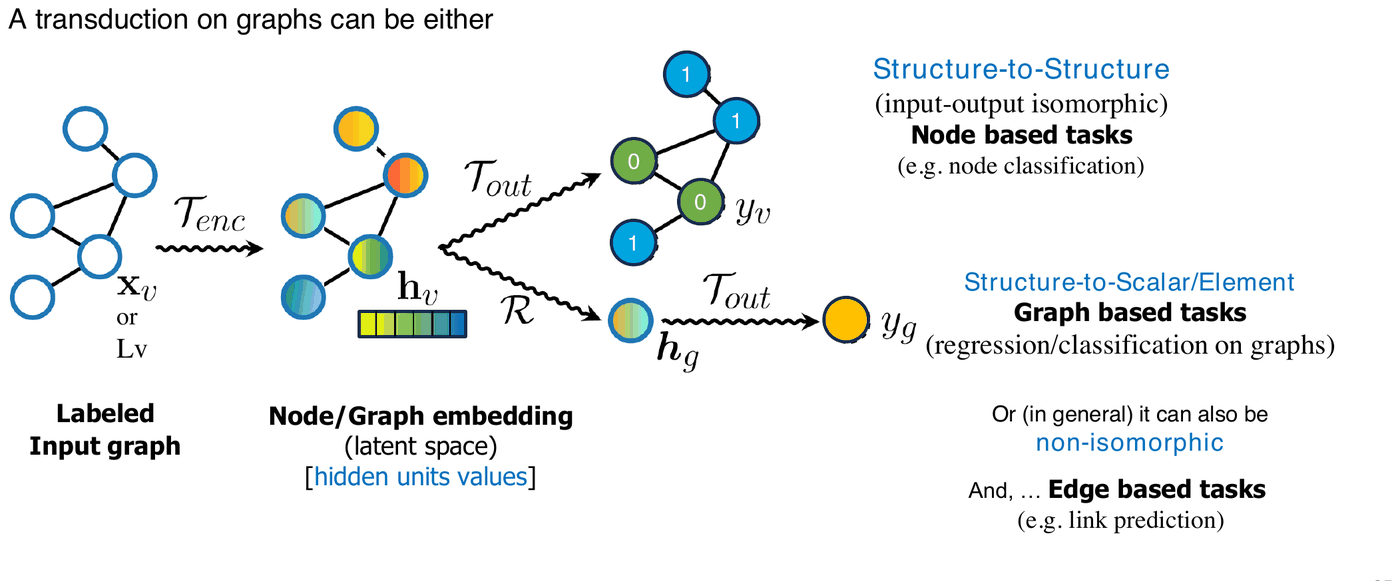
\includegraphics[width=0.89\linewidth,height=0.42\textheight,keepaspectratio]{images/21-sdl_trasduzioni.png}
\caption{Trasduzioni su grafi: il grafo viene codificato in un embedding dei
nodi, da cui si ottengono uscite per nodo o per l'intero grafo.}
\end{figure}

\begin{itemize}
\tightlist
\item
  \textbf{Struttura → struttura} (isomorfa input-output): compiti
  \textbf{a livello di nodo} (es. classificazione dei nodi).
\item
  \textbf{Struttura → scalare/elemento}: compiti \textbf{a livello di
  grafo} (regressione o classificazione di grafi).
\item
  In generale anche non isomorfa; e compiti \textbf{sugli archi} (es.
  \emph{link prediction}).
\end{itemize}

\subsection{Il message passing}\label{il-message-passing}

Come funziona una DGN? Il concetto astratto è il \textbf{message
passing}: i nodi ``parlano'' tra loro, scambiandosi messaggi per
informarsi a vicenda e diventare consapevoli della struttura
circostante.

\begin{enumerate}
\def\labelenumi{\arabic{enumi}.}
\tightlist
\item
  Ogni nodo calcola un \textbf{messaggio}, funzione della propria
  etichetta, dei vicini \(\mathcal{N}_v\) e degli archi tra loro, e lo
  invia ai vicini.
\item
  I nodi \textbf{aggregano} i messaggi ricevuti con una funzione
  \textbf{invariante per permutazione} (non importa l'ordine in cui
  arrivano).
\item
  Ogni nodo \textbf{aggiorna} i propri attributi (lo \textbf{stato})
  combinando i messaggi con i parametri liberi \(W\).
\end{enumerate}

\begin{figure}[htbp]
\centering
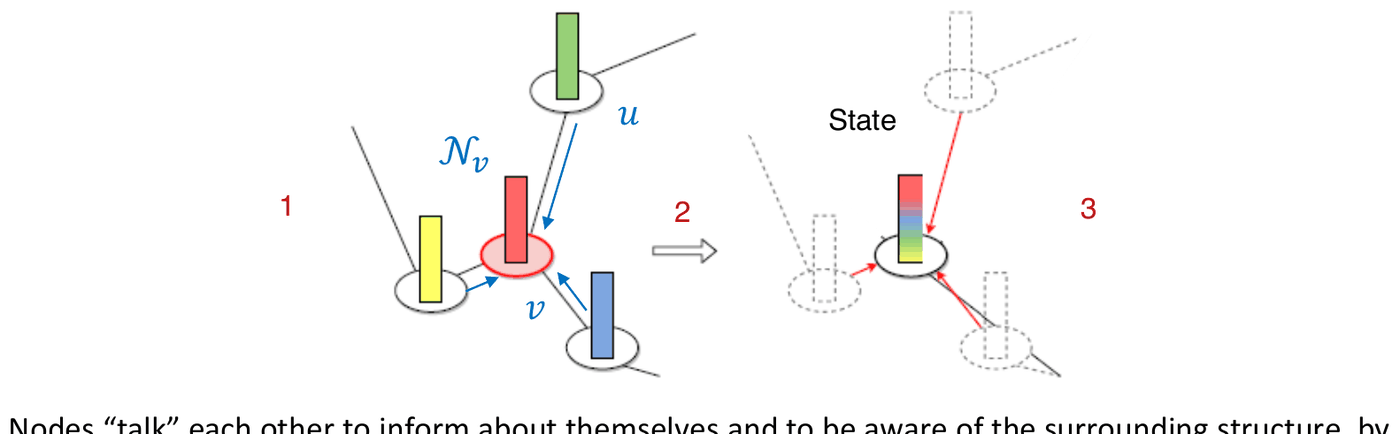
\includegraphics[width=0.80\linewidth,height=0.42\textheight,keepaspectratio]{images/21-sdl_message-passing.png}
\caption{Il message passing: messaggi dai vicini, aggregazione, aggiornamento
dello stato.}
\end{figure}

Lo stato non dipende solo dal vicinato locale: \textbf{iterando} il
message passing, l'informazione si \textbf{diffonde} da ogni nodo a
tutti gli altri. Infine si può emettere un'uscita \textbf{per ogni
nodo}, oppure \textbf{per l'intero grafo} tramite un'aggregazione
invariante per permutazione delle rappresentazioni dei nodi, detta
\textbf{global pooling} (ad esempio somma o media).

\subsection{Il legame con le CNN}\label{il-legame-con-le-cnn}

Sia le CNN sia le reti convoluzionali per grafi visitano ogni nodo dei
dati, ma:

\begin{itemize}
\tightlist
\item
  nella \textbf{CNN} il kernel convoluzionale si applica su una
  \textbf{griglia regolare} 2D: si fa una media pesata dei pixel nella
  finestra, e i vicini di un pixel sono \textbf{ordinati} e in
  \textbf{numero fisso};
\item
  nei \textbf{grafi} la CNN non si applica direttamente: i vicini di un
  vertice sono \textbf{non ordinati} e in \textbf{numero variabile}. Si
  limita il campo recettivo ai \textbf{vicini}, si usa la
  \textbf{condivisione dei pesi} in modo invariante per permutazione
  (astraendo da qualunque ordinamento dei nodi), e si estende il
  vicinato locale tramite la \textbf{stratificazione}.
\end{itemize}

\begin{figure}[htbp]
\centering
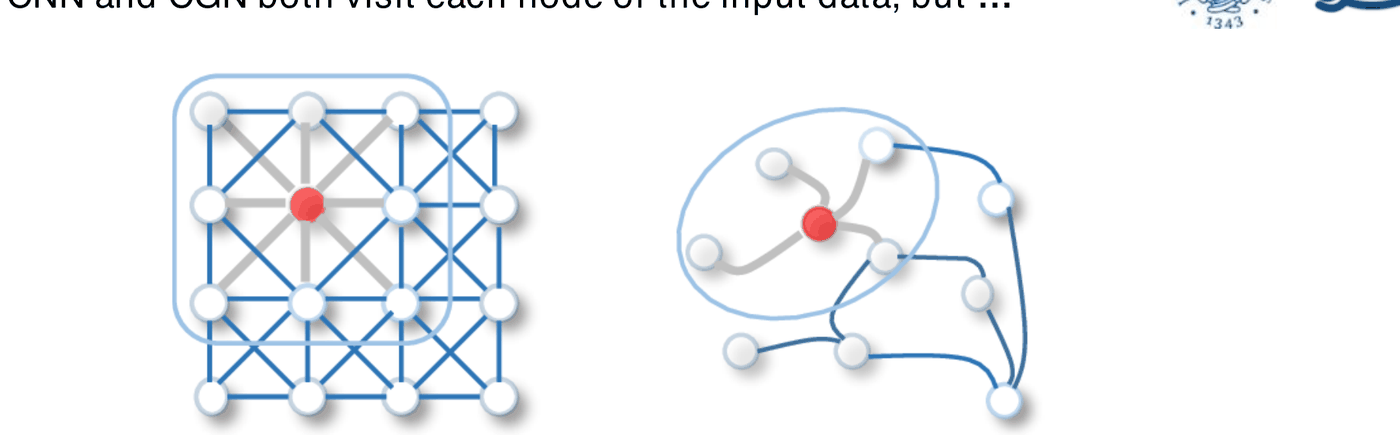
\includegraphics[width=0.80\linewidth,height=0.42\textheight,keepaspectratio]{images/21-sdl_cnn-vs-grafi.png}
\caption{Convoluzione su griglia (CNN) e su grafo.}
\end{figure}

\subsection{La formula generale}\label{la-formula-generale}

Il message passing si itera sugli strati (o iterazioni) \(l\): \[
\mathbf{h}_v^{(l)} = AGG_{W^{(l)}}\Big(\mathbf{L}_v,\; \mathbf{h}_v^{(l-1)},\; \{\mathbf{h}_u^{(l-1)} : u \in \mathcal{N}(v)\}\Big), \qquad l = 1, \dots, L,
\] dove \(AGG\) aggrega (propaga) i messaggi dai vicini \(u\) con un
operatore \textbf{invariante per permutazione} sull'insieme dei vicini
(es. una somma) e combinazioni delle attivazioni delle unità, \(W\) sono
i parametri liberi, \(\mathbf{L}_v\) l'etichetta del nodo, e
\(\mathcal{N}\) è dato dalla matrice di adiacenza \(A\). Applicare
questo calcolo a ogni nodo corrisponde a una \textbf{visita parallela e
non ordinata} del grafo a ogni iterazione.

Ci sono molte varianti:

\begin{itemize}
\tightlist
\item
  \textbf{GCN} (Kipf, Welling, 2017):
  \(\mathbf{h}^{(l)} = \text{ReLU}\big(\hat{A}\,\mathbf{h}^{(l-1)}W^{(l)}\big)\),
  con \(\hat A\) la matrice di adiacenza normalizzata per grado;
\item
  \textbf{GraphConv} (Morris et al., 2019):
  \(\mathbf{h}^{(l)} = f\big(W_1^{(l)}\mathbf{h}^{(l-1)} + W_2^{(l)}A\,\mathbf{h}^{(l-1)}\big)\);
\item
  \textbf{GAT} (Veličković et al., 2018): aggregazione basata
  sull'\textbf{attenzione}.
\end{itemize}

(Molte sono disponibili in \emph{PyTorch Geometric}.)

\begin{boxtip}{Perché è rilevante per il deep learning}

Le DGN sono \textbf{intrinsecamente profonde}: il processo non è locale.
Iterando sugli strati, le rappresentazioni latenti dei nodi includono
progressivamente l'informazione \textbf{contestuale} di nodi sempre più
lontani (diffusione).

\end{boxtip}

\begin{figure}[htbp]
\centering
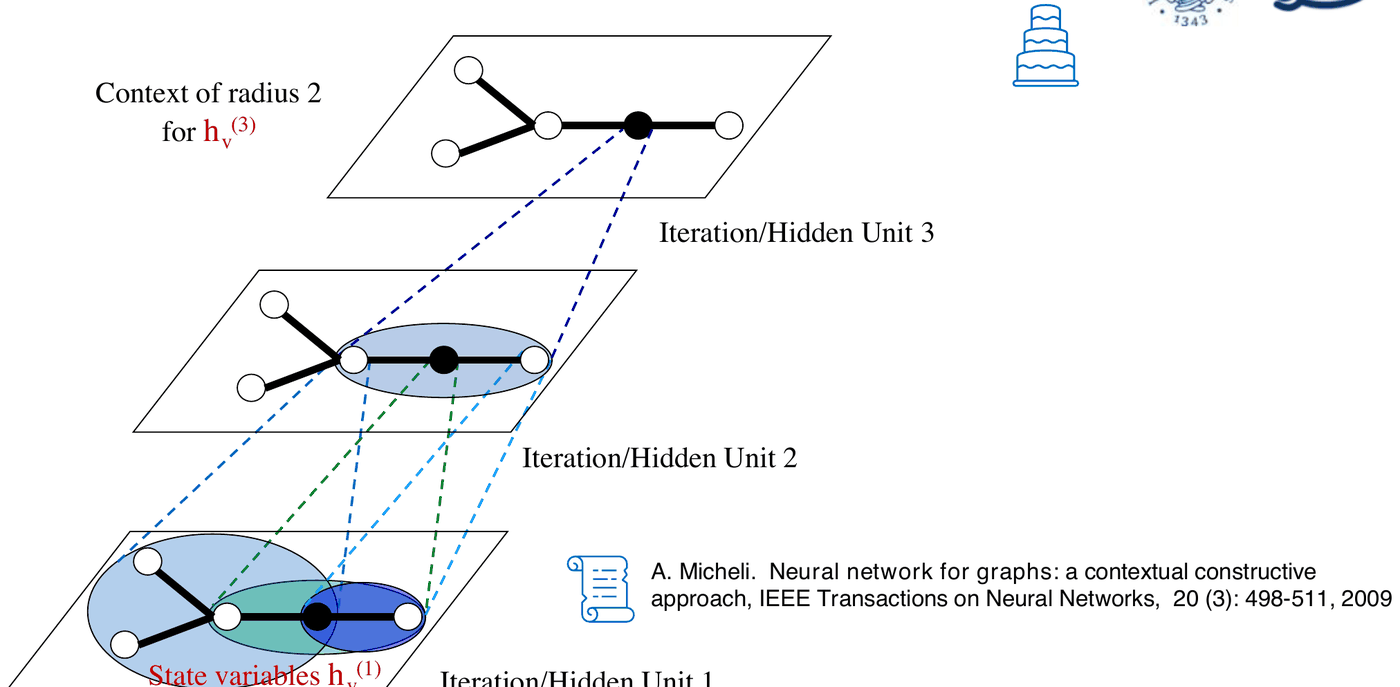
\includegraphics[width=0.86\linewidth,height=0.42\textheight,keepaspectratio]{images/21-sdl_contesto.png}
\caption{Evoluzione del contesto (composizionale) attraverso le iterazioni: al
terzo strato lo stato del nodo ha un contesto di raggio 2.}
\end{figure}

\subsection{NN4G e GCN: iterazioni come
strati}\label{nn4g-e-gcn-iterazioni-come-strati}

\begin{figure}[htbp]
\centering
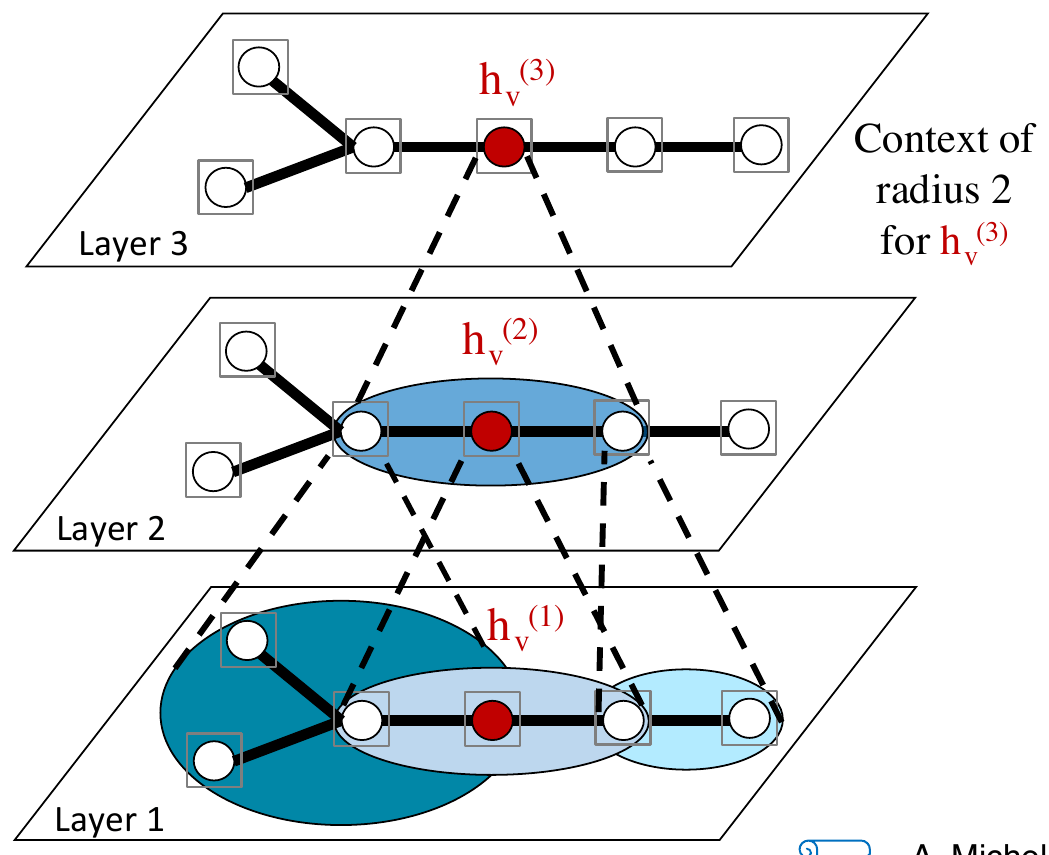
\includegraphics[width=0.49\linewidth,height=0.42\textheight,keepaspectratio]{images/21-sdl_nn4g.png}
\caption{GCN e NN4G: ogni iterazione del message passing è un nuovo strato.}
\end{figure}

Nelle reti convoluzionali per grafi (GCN, NN4G), \textbf{ogni iterazione
del message passing è un nuovo strato}, e per ogni nodo il contesto si
\textbf{compone} attraverso gli strati:

\begin{itemize}
\tightlist
\item
  il \textbf{campo recettivo} si estende incrementalmente all'aumentare
  degli strati;
\item
  la \textbf{profondità è funzionale alla crescita del contesto};
\item
  addestrando il modello si impara \textbf{come rappresentare il grafo}:
  end-to-end per le GCN generali, \textbf{strato per strato} (in modo
  incrementale) per NN4G, con numero di strati automatico e senza
  problemi di vanishing gradient.
\end{itemize}

\textbf{NN4G} (Micheli, 2009) calcola una variabile di stato per ogni
strato e ogni vertice: \[
h_v^{(1)} = f\left(\sum_{j=0}^{|L_v|}\bar w_{1j}\,L_j(v)\right), \qquad h_v^{(l)} = f\left(\underbrace{\sum_{j=0}^{|L_v|}\bar w_{lj}\,L_j(v)}_{\text{etichetta di } v} + \underbrace{\sum_{j=1}^{l-1}\hat w_{lj}\sum_{u \in \mathcal{N}(v)}h_u^{(j)}}_{\text{contesto dai vicini, da tutti gli strati precedenti}}\right), \quad l = 2, \dots, N.
\] Non è ricorsivo: ogni strato usa gli stati degli strati
\textbf{precedenti}. Le unità si aggiungono una alla volta (in stile
Cascade Correlation), e le uscite dei vari strati vengono combinate per
produrre il risultato sul grafo.

\subsection{GNN e GraphESN: approccio
ricorsivo}\label{gnn-e-graphesn-approccio-ricorsivo}

Negli approcci \textbf{ricorsivi} (GNN, GraphESN) il processo di
diffusione è simile, ma \(l\) è il numero di \textbf{iterazioni sullo
stesso strato} (o strati con pesi condivisi). È un \textbf{sistema
dinamico}: tipicamente si richiede la \textbf{convergenza a un punto
fisso}, usato come embedding del grafo, e per questo si vincola la
dinamica del message passing a essere \textbf{contrattiva}.

\begin{itemize}
\tightlist
\item
  \textbf{GNN} (Scarselli et al., 2009): con addestramento
  dell'embedding.
\item
  \textbf{GraphESN} (Gallicchio, Micheli, 2010): estende le Echo State
  Network: la funzione di message passing \textbf{non è addestrata} (è
  un reservoir casuale), ma si controllano direttamente i parametri del
  sistema dinamico.
\end{itemize}

\[
\mathbf{h}_v^{(l)} = \tanh\left(\sum_{j=0}^{|L_v|}\bar w_{lj}\,L_j(v) + \sum_{u \in \mathcal{N}(v)}\hat W\,\mathbf{h}_u^{(l-1)}\right),
\] iterata fino a convergenza; l'uscita per un grafo si ottiene con un
global pooling \(X\) e un \textbf{readout lineare} addestrato con
pseudoinversa o ridge regression: \(y(g) = W_{out}\,X(\mathbf{h}(g))\).

\begin{figure}[htbp]
\centering
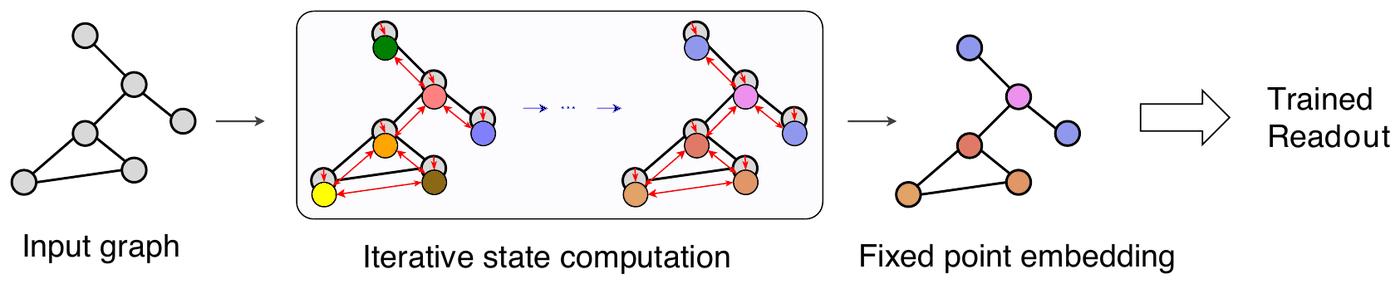
\includegraphics[width=0.80\linewidth,height=0.42\textheight,keepaspectratio]{images/21-sdl_gesn.png}
\caption{GraphESN: calcolo iterativo degli stati fino a un embedding a punto
fisso, poi readout addestrato.}
\end{figure}

\section{Problemi aperti e alcune
proposte}\label{problemi-aperti-e-alcune-proposte}

\begin{figure}[htbp]
\centering
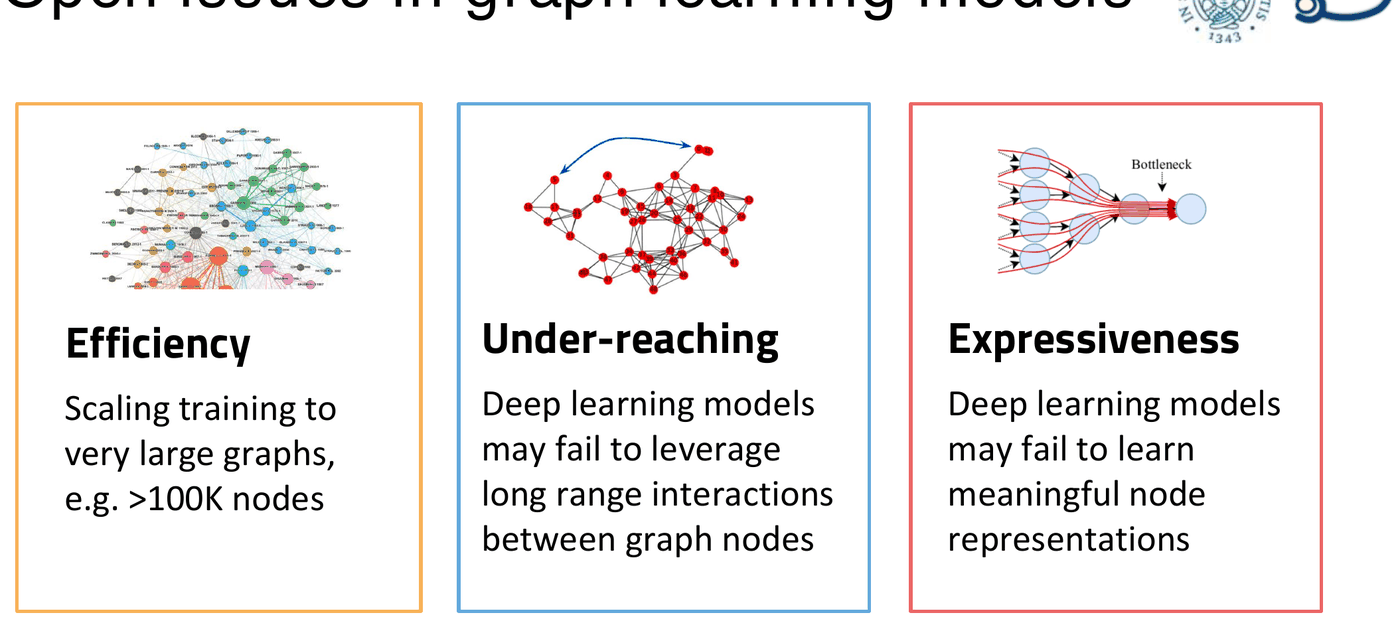
\includegraphics[width=0.86\linewidth,height=0.42\textheight,keepaspectratio]{images/21-sdl_problemi-aperti.png}
\caption{Problemi aperti nei modelli di apprendimento su grafi: efficienza,
under-reaching, espressività.}
\end{figure}

\subsection{Efficienza: oltre la backpropagation
end-to-end}\label{efficienza-oltre-la-backpropagation-end-to-end}

\begin{itemize}
\tightlist
\item
  \textbf{GraphESN per la classificazione di nodi}: su grafi molto
  grandi (es. Twitch-gamers, 168.000 nodi) ottiene un'accuratezza pari o
  superiore alla maggior parte dei modelli addestrati end-to-end, con
  un'accelerazione fino a 10 volte, e l'addestramento scala facilmente
  oltre i 100.000 nodi.
\item
  \textbf{NN4G+} (progettazione automatica dell'architettura): la rete
  si costruisce \textbf{incrementalmente}, con una doppia espansione
  sinergica. Si addestra \textbf{un'unità alla volta} (niente
  backpropagation end-to-end attraverso gli strati); uno strato viene
  espanso finché l'accuratezza di validazione migliora, e si aggiungono
  nuovi strati finché migliora. Le architetture ottenute sono adattate
  al task, costantemente più profonde e snelle rispetto a una ricerca
  esplicita dell'architettura, e vengono costruite in minuti invece che
  ore (oltre 10 volte più veloce, senza perdita di accuratezza).
\end{itemize}

\subsection{I problemi della profondità: gli
``over-*''}\label{i-problemi-della-profondituxe0-gli-over-}

La profondità serve, ma il message passing ha dei bias e dei problemi:

\begin{itemize}
\tightlist
\item
  \textbf{Over-smoothing} (Li et al., 2018): l'accuratezza tipicamente
  cala oltre 4--5 strati; le rappresentazioni dei nodi
  \textbf{collassano} negli strati profondi. Il message passing agisce
  come una \textbf{diffusione}, e le rappresentazioni di alto livello
  dei nodi diventano tutte simili.
\item
  \textbf{Over-squashing} (Alon, Yahav, 2021): è un \textbf{collo di
  bottiglia}. Il campo recettivo cresce \textbf{esponenzialmente} con la
  profondità, ma tutta questa informazione va compressa in un embedding
  di dimensione fissa per nodo. La \textbf{sensibilità} della
  rappresentazione di un nodo alle feature di input di nodi lontani,
  misurata dallo Jacobiano
  \(\partial\mathbf{h}_v^{(L)}/\partial\mathbf{x}_u\), decresce
  esponenzialmente con il numero di strati.
\item
  Per l'addestramento end-to-end, la \textbf{difficoltà di
  retropropagare il gradiente} attraverso molti strati di message
  passing.
\end{itemize}

L'interazione tra questi fenomeni è un problema di ricerca aperto. Gli
effetti:

\begin{enumerate}
\def\labelenumi{\arabic{enumi}.}
\tightlist
\item
  \textbf{Under-reaching}: gli over-* impediscono di avere il campo
  recettivo necessario per apprendere interazioni tra nodi lontani.
\item
  \textbf{Eterofilia} nella classificazione dei nodi. Nei grafi
  \textbf{omofili} i nodi dello stesso vicinato condividono per lo più
  la stessa classe; nei grafi \textbf{eterofili} i nodi della stessa
  classe sono generalmente lontani, e le predizioni basate soprattutto
  sui vicini immediati possono essere fuorvianti. Sono task
  potenzialmente difficili per il message passing standard, per via
  degli over-* e del bias verso grafi ``omogenei''.
\end{enumerate}

\begin{figure}[htbp]
\centering
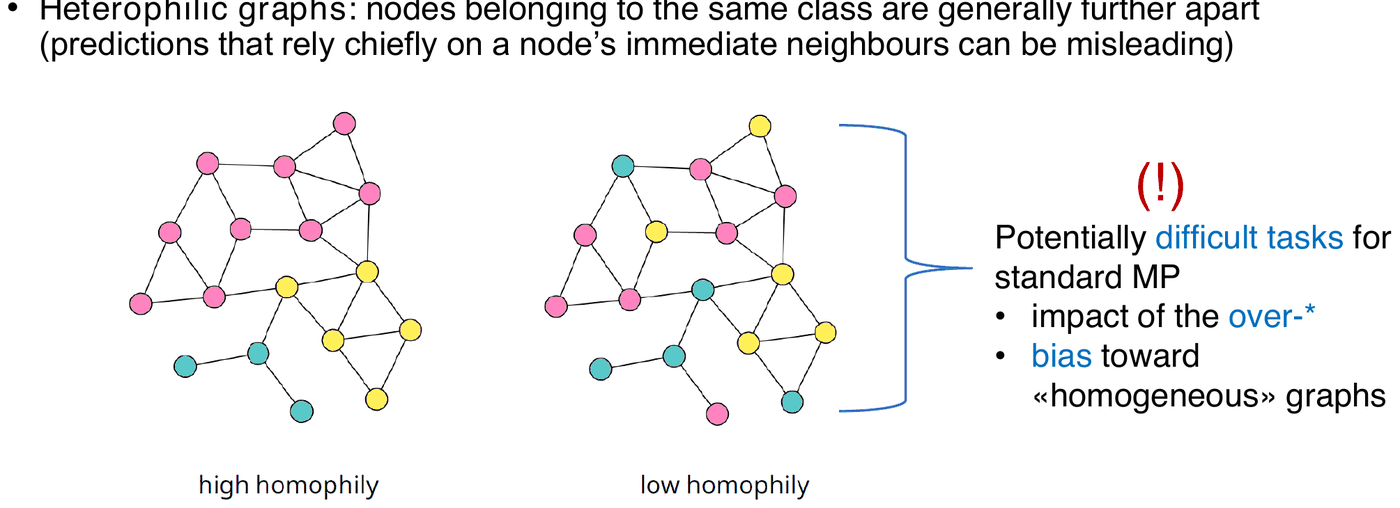
\includegraphics[width=0.80\linewidth,height=0.42\textheight,keepaspectratio]{images/21-sdl_eterofilia.png}
\caption{Grafi ad alta e bassa omofilia: i secondi sono difficili per il message
passing standard.}
\end{figure}

\subsubsection{Strumenti per l'analisi}\label{strumenti-per-lanalisi}

\begin{itemize}
\tightlist
\item
  \textbf{Modelli che separano il bias del message passing dai problemi
  dell'addestramento end-to-end}: NN4G (incrementale, senza propagare il
  gradiente attraverso gli strati) e GraphESN (nessun addestramento
  dell'embedding, controllo diretto della norma spettrale \(\|W\|\),
  cioè della costante di Lipschitz della funzione di message passing
  ricorsiva). Poiché \[
  \left\|\frac{\partial\mathbf{h}_v^{(L)}}{\partial\mathbf{x}_u}\right\| \le \prod_{l=1}^{L}\|W^{(l)}\|\cdot\big(A^L\big)_{u,v},
  \] imporre \(\|W\| > 1\) impedisce che la sensibilità rispetto
  all'input svanisca esponenzialmente (over-squashing).
\item
  \textbf{Analisi spettrale} degli strati. La ``frequenza'' su un grafo
  è la variabilità del segnale (etichette, embedding) tra nodi vicini.
  L'\textbf{energia di Dirichlet}
  \(E(\mathbf{h}) = \sum_{v}\sum_{u \in \mathcal{N}_v}\|\mathbf{h}_v - \mathbf{h}_u\|^2\)
  misura quanto il segnale varia sul grafo (visione spaziale) e, tramite
  la trasformata di Fourier su grafo (ottenuta dalla decomposizione del
  Laplaciano \(L = D - A\)), come la ``massa'' del segnale si
  distribuisce sullo spettro delle frequenze: un segnale a bassa
  frequenza (liscio) ha bassa energia. I grafi eterofili hanno segnali
  ad \textbf{alta frequenza}, e i task eterofili richiedono di
  \textbf{preservare le alte frequenze}.
\end{itemize}

Sul dataset \textbf{Chameleon} (una rete di pagine Wikipedia, 2277 nodi,
31.400 archi, omofilia 0,23), una ``prova da sforzo'' per l'eterofilia,
NN4G e GraphESN \textbf{preservano meglio l'energia} attraverso gli
strati, e mentre l'accuratezza degli altri modelli cala all'aumentare
del message passing, la loro no. In un esperimento con 12 strati:
GraphESN 73,7\%, NN4G 68,3\%, GCN 57,8\%, GAT 55,0\%, GraphConv 33,8\%.

\subsection{Estensioni in corso}\label{estensioni-in-corso}

\begin{itemize}
\tightlist
\item
  \textbf{Grafi dinamici/temporali}: relazioni o valori dei nodi che
  evolvono nel tempo (diffusione di infezioni, contenuti sui social,
  segnali sui nodi). Le \textbf{Dynamic Graph Echo State Network}
  realizzano una convoluzione spazio-temporale con un reservoir
  multistrato, efficaci quanto le reti temporali per grafi addestrate
  completamente, ma con un'accelerazione di 100 volte nell'addestramento
  e 10 nell'inferenza.
\item
  \textbf{Generazione di grafi}: apprendere la distribuzione \(p(G)\) di
  un insieme di grafi per campionarne di nuovi (es. generazione di
  molecole basata su frammenti), utile per equità, robustezza, privacy.
\item
  \textbf{Spiegabilità} (XAI) per le reti su grafi: ad esempio
  identificare gli anelli benzenici che determinano una classificazione,
  o i frammenti strutturali noti (come l'accettore di Michael) che
  influenzano l'attivazione del pathway P53 nei dati Tox21.
\item
  \textbf{Network quantification}: predire la \textbf{prevalenza} delle
  classi tra i nodi non etichettati invece di classificarli
  singolarmente (voto, ricerche di mercato, epidemiologia).
\item
  \textbf{Bioinformatica}: predire proprietà dinamiche (robustezza,
  sensitività) di pathway biochimici e reti di interazione
  proteina-proteina rappresentati come grafi.
\end{itemize}

\section{Altri approcci: i kernel per
strutture}\label{altri-approcci-i-kernel-per-strutture}

I \textbf{metodi kernel} si estendono facilmente a grafi di tipi diversi
(sequenze, alberi, grafi orientati o no, ciclici o aciclici), perché
basta definire un prodotto scalare
\(k(x, x') = \langle\phi(x), \phi(x')\rangle\), cioè una
\textbf{similarità} tra dati di qualsiasi tipo, con un embedding
implicito in uno spazio euclideo.

\begin{itemize}
\tightlist
\item
  \textbf{Kernel marginalizzati}: la similarità tra due grafi si basa
  sui cammini di etichette comuni ottenuti con random walk; il kernel è
  il prodotto scalare dei vettori di conteggio, mediato su tutti i
  possibili cammini. Il costo scala tipicamente in modo quadratico con
  la dimensione del grafo.
\item
  \textbf{Kernel di convoluzione}: si decompongono gli oggetti in
  \textbf{sotto-strutture} e si definisce il kernel combinando kernel
  tra le sotto-strutture.
\end{itemize}

\begin{figure}[htbp]
\centering
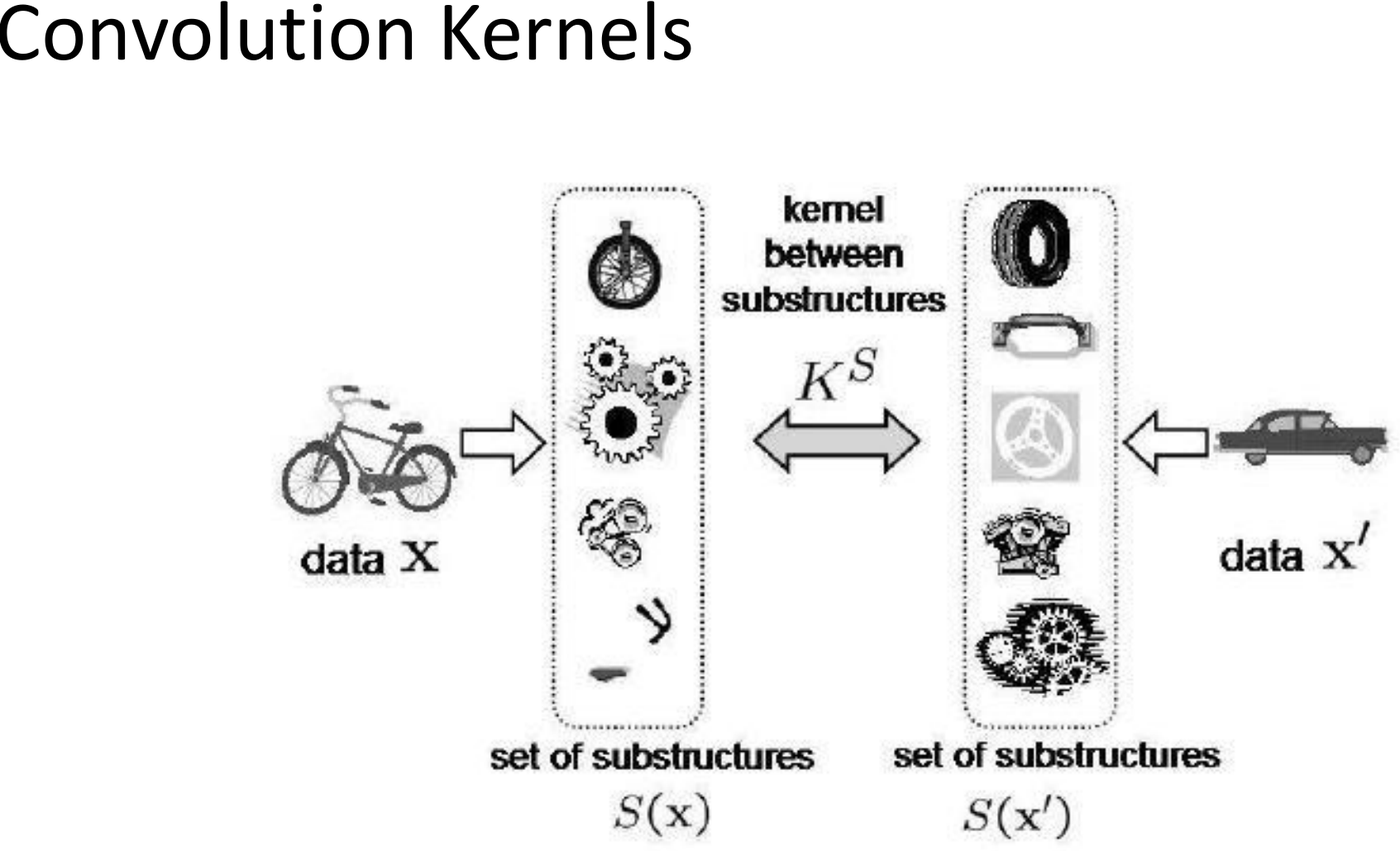
\includegraphics[width=0.63\linewidth,height=0.42\textheight,keepaspectratio]{images/21-sdl_convolution-kernel.png}
\caption{Kernel di convoluzione: la similarità tra oggetti si calcola a partire
dalla similarità tra le loro sotto-strutture.}
\end{figure}

\begin{boxwarning}{Limiti dei kernel per strutture}

\begin{itemize}
\tightlist
\item
  \textbf{Efficienza}: il costo è critico, per via della scomposizione
  in sotto-strutture.
\item
  \textbf{Adattività}: sono metodi guidati dalla conoscenza, con una
  misura di similarità \textbf{fissata prima dell'apprendimento}: la
  codifica nello spazio delle feature non è appresa. Il vantaggio è
  poter sfruttare la conoscenza a priori per un problema specifico.
\item
  Per i domini strutturati \textbf{non si conosce l'universalità}: la
  scelta del kernel è critica, e calcolare un kernel \textbf{completo}
  per grafi è difficile almeno quanto il problema
  dell'\textbf{isomorfismo di grafi}. (Si studiano kernel adattivi.)
\end{itemize}

\end{boxwarning}

\begin{boxabstract}{Conclusioni}

\begin{itemize}
\tightlist
\item
  Si può fare deep learning su dati complessi \textbf{in modo
  efficiente}, senza un addestramento completamente end-to-end: modelli
  come GraphESN e NN4G costruiscono DGN accurate in modo efficiente e
  permettono di studiare il bias del message passing.
\item
  La \textbf{profondità} nelle DGN è necessaria (fa crescere il
  contesto), ma può causare problemi (over-smoothing, over-squashing,
  difficoltà di addestramento); andare oltre l'end-to-end può aiutare
  sia per l'efficienza sia per gli over-*.
\item
  Il ML per dati strutturati e grafi è una realtà concreta, ancora in
  sviluppo, che offre soluzioni nuove dove le \textbf{relazioni}
  contano. Se i dati hanno relazioni (seriali, gerarchiche, reti),
  \textbf{non conviene usare una rappresentazione piatta}. È anche una
  grande opportunità per trattare in modo uniforme tipi di dati diversi.
\end{itemize}

\end{boxabstract}

\begin{boxquestion}{Possibili domande d'esame}

\begin{itemize}
\tightlist
\item
  Perché trattare i dati strutturati direttamente, invece di
  trasformarli in vettori?
\item
  Quali tipi di trasduzione si possono definire sui grafi?
\item
  Descrivere il message passing e la formula generale delle DGN.
\item
  Differenza tra approcci a strati (GCN, NN4G) e ricorsivi (GNN,
  GraphESN).
\item
  Cosa sono over-smoothing e over-squashing? Cos'è l'eterofilia?
\item
  Pro e contro dei kernel per strutture.
\end{itemize}

\end{boxquestion}
